\section{Durchführung und Auswertung}

Es wurden vier Messungen bei $I \in {0,100,200,300}$ mA gemacht. Eine Messung startete stets bei großen Temperaturen; durch einen Unterdruck wurde auf $T=2,8$K runtergekühlt und schließlich wieder Helium eingelassen, sodass sich jeweils ein geschlossener Weg in der $R(T)$-Kurve bildet, die aufgenommen wurde. Die die angelegten Ströme sind dabei schon in den Betrag der induzierter Magnetfelder umgerechnet. Da es sich um eine einfache Helmholtzspule mit Radius $R=15$mm, Windungszahl $N=750$ handelt, gilt die Propertionalität

\begin{equation}
B(I) = \frac{4}{5}\sqrt{\frac{4}{5}} \frac{\mu_0 N}{R} I \equiv B_H I
\end{equation}

mit $B_H = 4,495 \cdot 10^{-2}$ T/A (Si-Einheiten, $\mu_0 = 1,2566\cdot 10^{-7}$ N/$A^2$).

\begin{figure}[h]
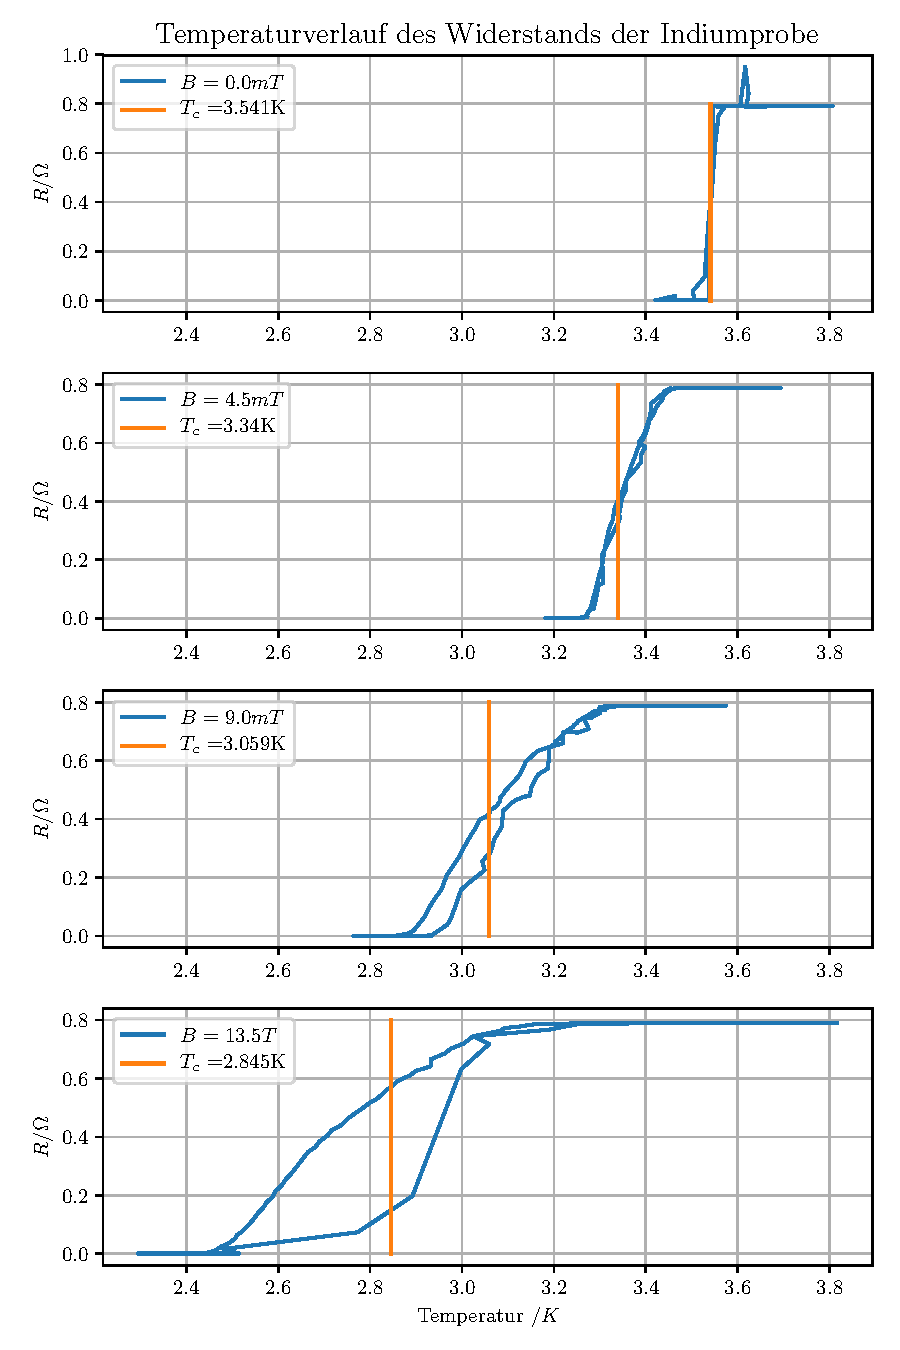
\includegraphics[width=\textwidth]{Temperaturverlauf_des_Widerstands_der_Indiumprobe.pdf}
\end{figure}

Die Graphen zeigen schön den sprunghaften Widerstandsabfall bei der jeweiligen Sprungtemperatur, wobei nur der Übergang bei $B=0$T wirklich als sprunghaft zu bezeichnen ist. In allen anderen Messungen erscheint der Phasenübergang sehr aufgeweitet, wobei wir Verunreinigungen in der Probe als Grund vermuten, die mit steigendem Magnetfeld immer stärker zum Tragen kommen. 


Mit folgender Näherungsgleichung für das Phasendiagramm können die kritischen B-Felder bei $T=0$ für die vier Messgrößen bestimmt werden:

\begin{equation}
B_c(T) = B_c(0) \cdot \left( 1 - \left( T / T_c(0) \right)^2 \right)
\end{equation}

Umgestellt nach $B_c(0) = B_i / (1 - (T / T_{c,0})^2 )$ ergibt das mit der Sprungtemperatur $T_c$ = $T_{c,0}$, die man aus der Tabelle abliest:

\begin{table}[h]
\center\begin{tabular}[h]{|r|r|r|l|l|}
\hline
$i$ & $I_i$ [mA] &  $B_i$ [mT] & $T_{c,i}$ [K] \\
\hline
0 &   0 &       0 & 3,541 \\
1 & 100 &  4,5 & 3,34 \\
2 & 200 &  9 & 3,059 \\
3 & 300 & 13,5 & 2,845 \\
\hline
\end{tabular}
\end{table}

Fittet man die Funktion an diese Werte, erhält man mit geeigneten Ausgangsparametern den Wert $T_c = 37,2 mT$ und damit das interpolierte Phasendiagramm:

\begin{figure}[h]
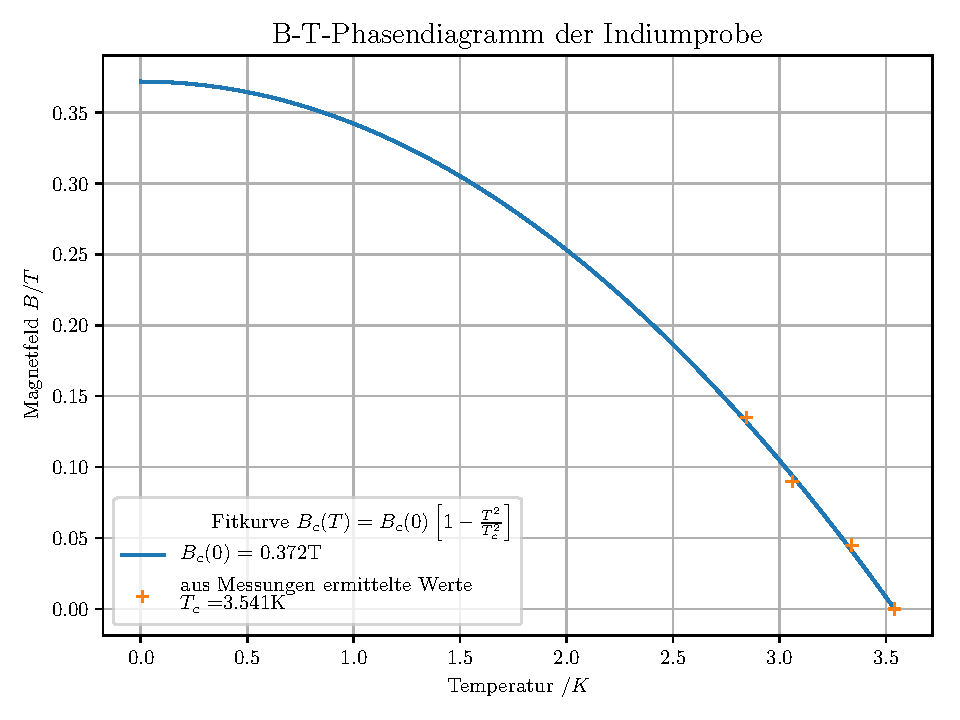
\includegraphics[width=\textwidth]{B-T-Phasendiagramm_der_Indiumprobe.pdf}
\end{figure}

Unser Fit passt wie am Phasendiagramm ersichtlich sehr gut zu den aufgenommenen Daten, und gibt einen guten Wert für das kritische Magnetfeld bei $T=0K$.
Das erweist auch der Vergleich mit dem Literaturwert $ T_{c,\textrm{Lit}} = 29,3\textrm{mT}$, zu dem wir natürlich eine Abweichung feststellen, aber uns durchaus in der richtigen Größenordnung bewegen. 

